\chapter{Alternative Öffnungsmöglichkeiten}
Dieses Kapitel behandelt die Einbindung des Sprachassistenten, der Weboberfläche, des RFID-Moduls, des Ultraschallsensors und den praktischen Aufbau und Verkabelung aller Module.

\section{Sprachassistenten-Steuerung}
Zunächst wurde versucht den Sprachassisten Alexa von Amazon an den Raspberry Pi anzubinden. Die entsprechenden Bibliotheken konnten zwar installiert werden, auf der Developer-Oberfläche von Amazon erschienen allgemeine Fehlermeldungen die keinem konkreten Problem zuzuordnen waren. Die Verbindung zur Software auf dem Raspberry Pi konnte aber nachgewiesen werden, sodass wir von einer fehlerhaften Syntax der übertragenen Inhalte ausgehen, vermutlich durch Versionskonflikte.
Eine Alterative Lösung mit Google Home schien zunächst sehr vielversprechend, da Goolge in der Dokumentation ebenfalls einen Raspberry Pi als Einrichtungsbeispiel verwendet. Es stellte sich jedoch heraus, dass auch hier trotz orndungsgemäßem Befolgen der Anleitung keine Verbindung zustande kam. Die erhaltenen Fehlermeldungen ließen auf ein Paketproblem in der verwendeten Betriebssytemversion zu, die wird schlussendlich nicht lösen konnten. % TODO Anhang
Als Workaround wurde ein Alexa WiFi-Relais beschafft, das sich mit der App eines Drittanbieters (eWeLink) verbinden und dann in die Alexa-Umgebung integrieren lässt. Dieses Modul wurde nun so angeschlossen, dass es bei Aktivierung einen \ac{GPIO}-PIN mit 3.3V Spannung versorgt. Dieser Vorgang kann wiederum mit einer einfachen Schleife in einem Python Skript auf dem RasPi abgefragt werden und weitere Aktionen wie logging etc. ausgeführt werden. Prinzipiell wäre auch ein einfacherer, direkter Anschluss des Relais an den Garagentoröffner in Parallelschaltung möglich gewesen. Auf diesen wurde aber aus Kontroll- und Sicherheitsgründen verzichtet.

\section{Weboberfläche}
Da die Implementierung im Rahmen des Projekts auf einem Raspberry Pi stattfindet und Python bereits für viele Anwendungen innerhalb des Projekts verwendet wird, wird sich für das in Python geschriebene Webframework Flask entschieden. Dies hat den Vorteil, dass andere Komponenten, die bereits in Python geschrieben sind, direkt ohne Mehraufwand in die Weboberfläche integriert werden können.

Daher wird im Rahmen des Projekts für die Realisierung einer Weboberfläche eine einfache FlaskApp erstellt, die den üblichen Aufbau hat mit einer flaskapp.py, die die Weboberfläche steuert, und auf einzelne Templates, die wiederum in HTML geschrieben werden, zugreift. Hierbei wird in der flaskapp.py-Datei die Initialisierung der Weboberfläche sowie das Routing und dem Datentransfer zwischen den Seiten festgelegt sowie auch die Funktion, die die Garage öffnet. Als Templates die als Seite geladen werden, wird eines für die Startseite erstellt und eines für die Seite, auf der die Logs angezeigt werden sollen. Die Hauptseite, die bei Aufruf der Seite geladen wird, enthält einen Button, der mittels der in der flaskapp.py dafür festgelegten Funktion die SmartGarage öffnet und einen Eintrag in der Logs-Datei erstellt. Des Weiteren enthält diese Seite die Information ob in der Garage ein Fahrzeug steht, oder nicht. Dies geschieht über die Ultraschallmessung, wie bereits zuvor erläutert. Ebenfalls wird von dieser Seite aus auf die Logs-Seite verlinkt. Die Logs-Seite bezieht die Daten aus der Logs-Datei und gibt diese auf der Weboberfläche aus, wodurch der Besitzer der Garage die geloggten Öffnungen einsehen kann.

\section{RFID}

Die Implementierung eines RFID-Systems in der SmartGarage bietet eine weitere Möglichkeit die Garage zu öffnen. Für das Projekt wurde daher ein RFID-RC522 Modul an den Raspberry Pi angeschlossen, welches als Lesegerät Transponder auslesen kann. Angesteuert vom Raspberry Pi wird das Modul mittels der GPIO-Ports ähnlich wie beispielsweise bereits dem Ultraschallsensors. Das Auslesen wird dann mit Hilfe eines Python-Skripts gesteuert und mit einer Whitelist abgeglichen.
Trotz der komplexen Technik gelang der Anschluss dank eines online verfügbaren Tutorials problemlos.\autocite[Vgl.][]{tutorialrfikd}
Als Transponder kann im Projekt jede beschreibbare RFID-Karte oder RFID-Chipkarte verwendet werden, solange diese die vorausgesetzte Frequenz von 13,56MHz unterstützt. Im Projekt wird hierfür eine RFID-Karte, die nicht mit dem richtigen Code beschriftet ist, als Beispiel für eine fehlerhafte Identifikation verwendet. 
Die großen Vorteile der RFID-Öffnungsmöglichkeit gegenüber z.B. einem Schlüssel sind die Protokollierbarkeit und die einfache und kostengünstige Sperrung falls ein Transponder geklaut oder verloren wird. In diesem Fall genügt es, den entsprechenden Eintrag aus der Whitelist zu entfernen. 


\section{Ultraschallsensor}
TODO voherigen Teil aufsplitten, Quelle

\section{Öffnungssimulation}
Um die Betätigung des Handsenders bei der Entwicklung simulieren und Testen zu können, wurde statt dem Relais zunächst eine LED an die GPIO-Pins des RasPi angeschlossen. Da die Lichtverhältnisse manchmal schwierig waren, wurde zusätzlich ein sogenannter aktiven Summer eingesetzt. Dieser erklingt dann zum Beispiel, wenn der richtige RFID Chip an das Lesegerät gehalten wird und somit die Garage geöffnet oder geschlossen wird. Dabei handelt es sich um einen Oszillator der, wird er einer gewissen Spannung untersetzt, anfängt zu Vibrieren und damit ein Ton erzeugt. Ausgeführt und koordiniert wird der Buzzer über ein Simples Python Skript das mittels der Bibliothek GPIO (General-Purpose Input/Output) in der Lage ist den Buzzer an oder auszuschalten. Dabei wird durch einen definierten Port, in diesem Fall „Port 4“, mittels einer $for$ Schleife die Spannung je nach $positivem$ oder $negativem$ Signal Ton koordiniert und eine andere Tonsequenz abgespielt.

Zu Präsentationszwecken wurde der Code zum Aktivieren der LED bzw. des Buzzers dann durch einen anderen ersetzt, der per SSH auf einen zweiten Raspberry Pi zugreift und dort ein Video eines öffnenden und schließenden Garagentors abspielt.
Dabei wird lokal eine Binärvariable geändert um den Zustand des Garagentors (offen oder geschlossen) speichert und das richtige Video auswählt.
Jedoch funktioniert diese Lösung nicht ganz zuverlässig, da nach jedem Zugriff das Video des vorherigen Versuchs trotz geschlossener SSH-Verbindung offen bleibt. 


\section{Steckplan}

Auf Abbildung \ref{Steckplansm} ist die schlussendlich verwendete Steckung abgebildet. Hierbei war zu beachten, dass die im Internet verfügbaren Anleitungen und Tutorials nicht unbedingt miteinander kompatibel sind und einige \ac{GPIO}-Pins von mehreren Vorlagen verwendet werden. Hier muss demetsprechend ein anderer freier Pin mit gleicher I/O-Funktion gefunden werden und der Code angepasst werden. Außerdem ist die Spannung zwingend zu beachten. Manche Module, wie der Ultraschallsensor, benötigen eine Spannung von 5V, andere nur 3.3V. Die GPIO-Pins des Raspberry Pi, sind auf 3.3V ausgelegt und nicht vor Überspannug geschützt. Ein versehentliches Verbinden der beiden Spannungsnetze kann zu irreperablen Hardwareschäden führen. Deshalb wurde beispielsweie am Ultraschallsensor ein Spannungsteiler eingebaut.

Der zur Steckung gehörige elektrische Schaltplan findet sich in Anhang \ref{Schaltplan}.
Auf Abbild \ref{Aufbau1} ist der Aufbau in der Praxis abgebildet. Das Objekt rechts auf dem Bild ist ein 4G-Router, der aufgrund der schlechten Internetverbindung bei Gruppenarbeiten vor Ort benötigt wurde.
Weitere Bilder des Versuchsaufbaus in Anhang \ref{Aufbauanhang}
\begin{figure}[H]
	\centering 
	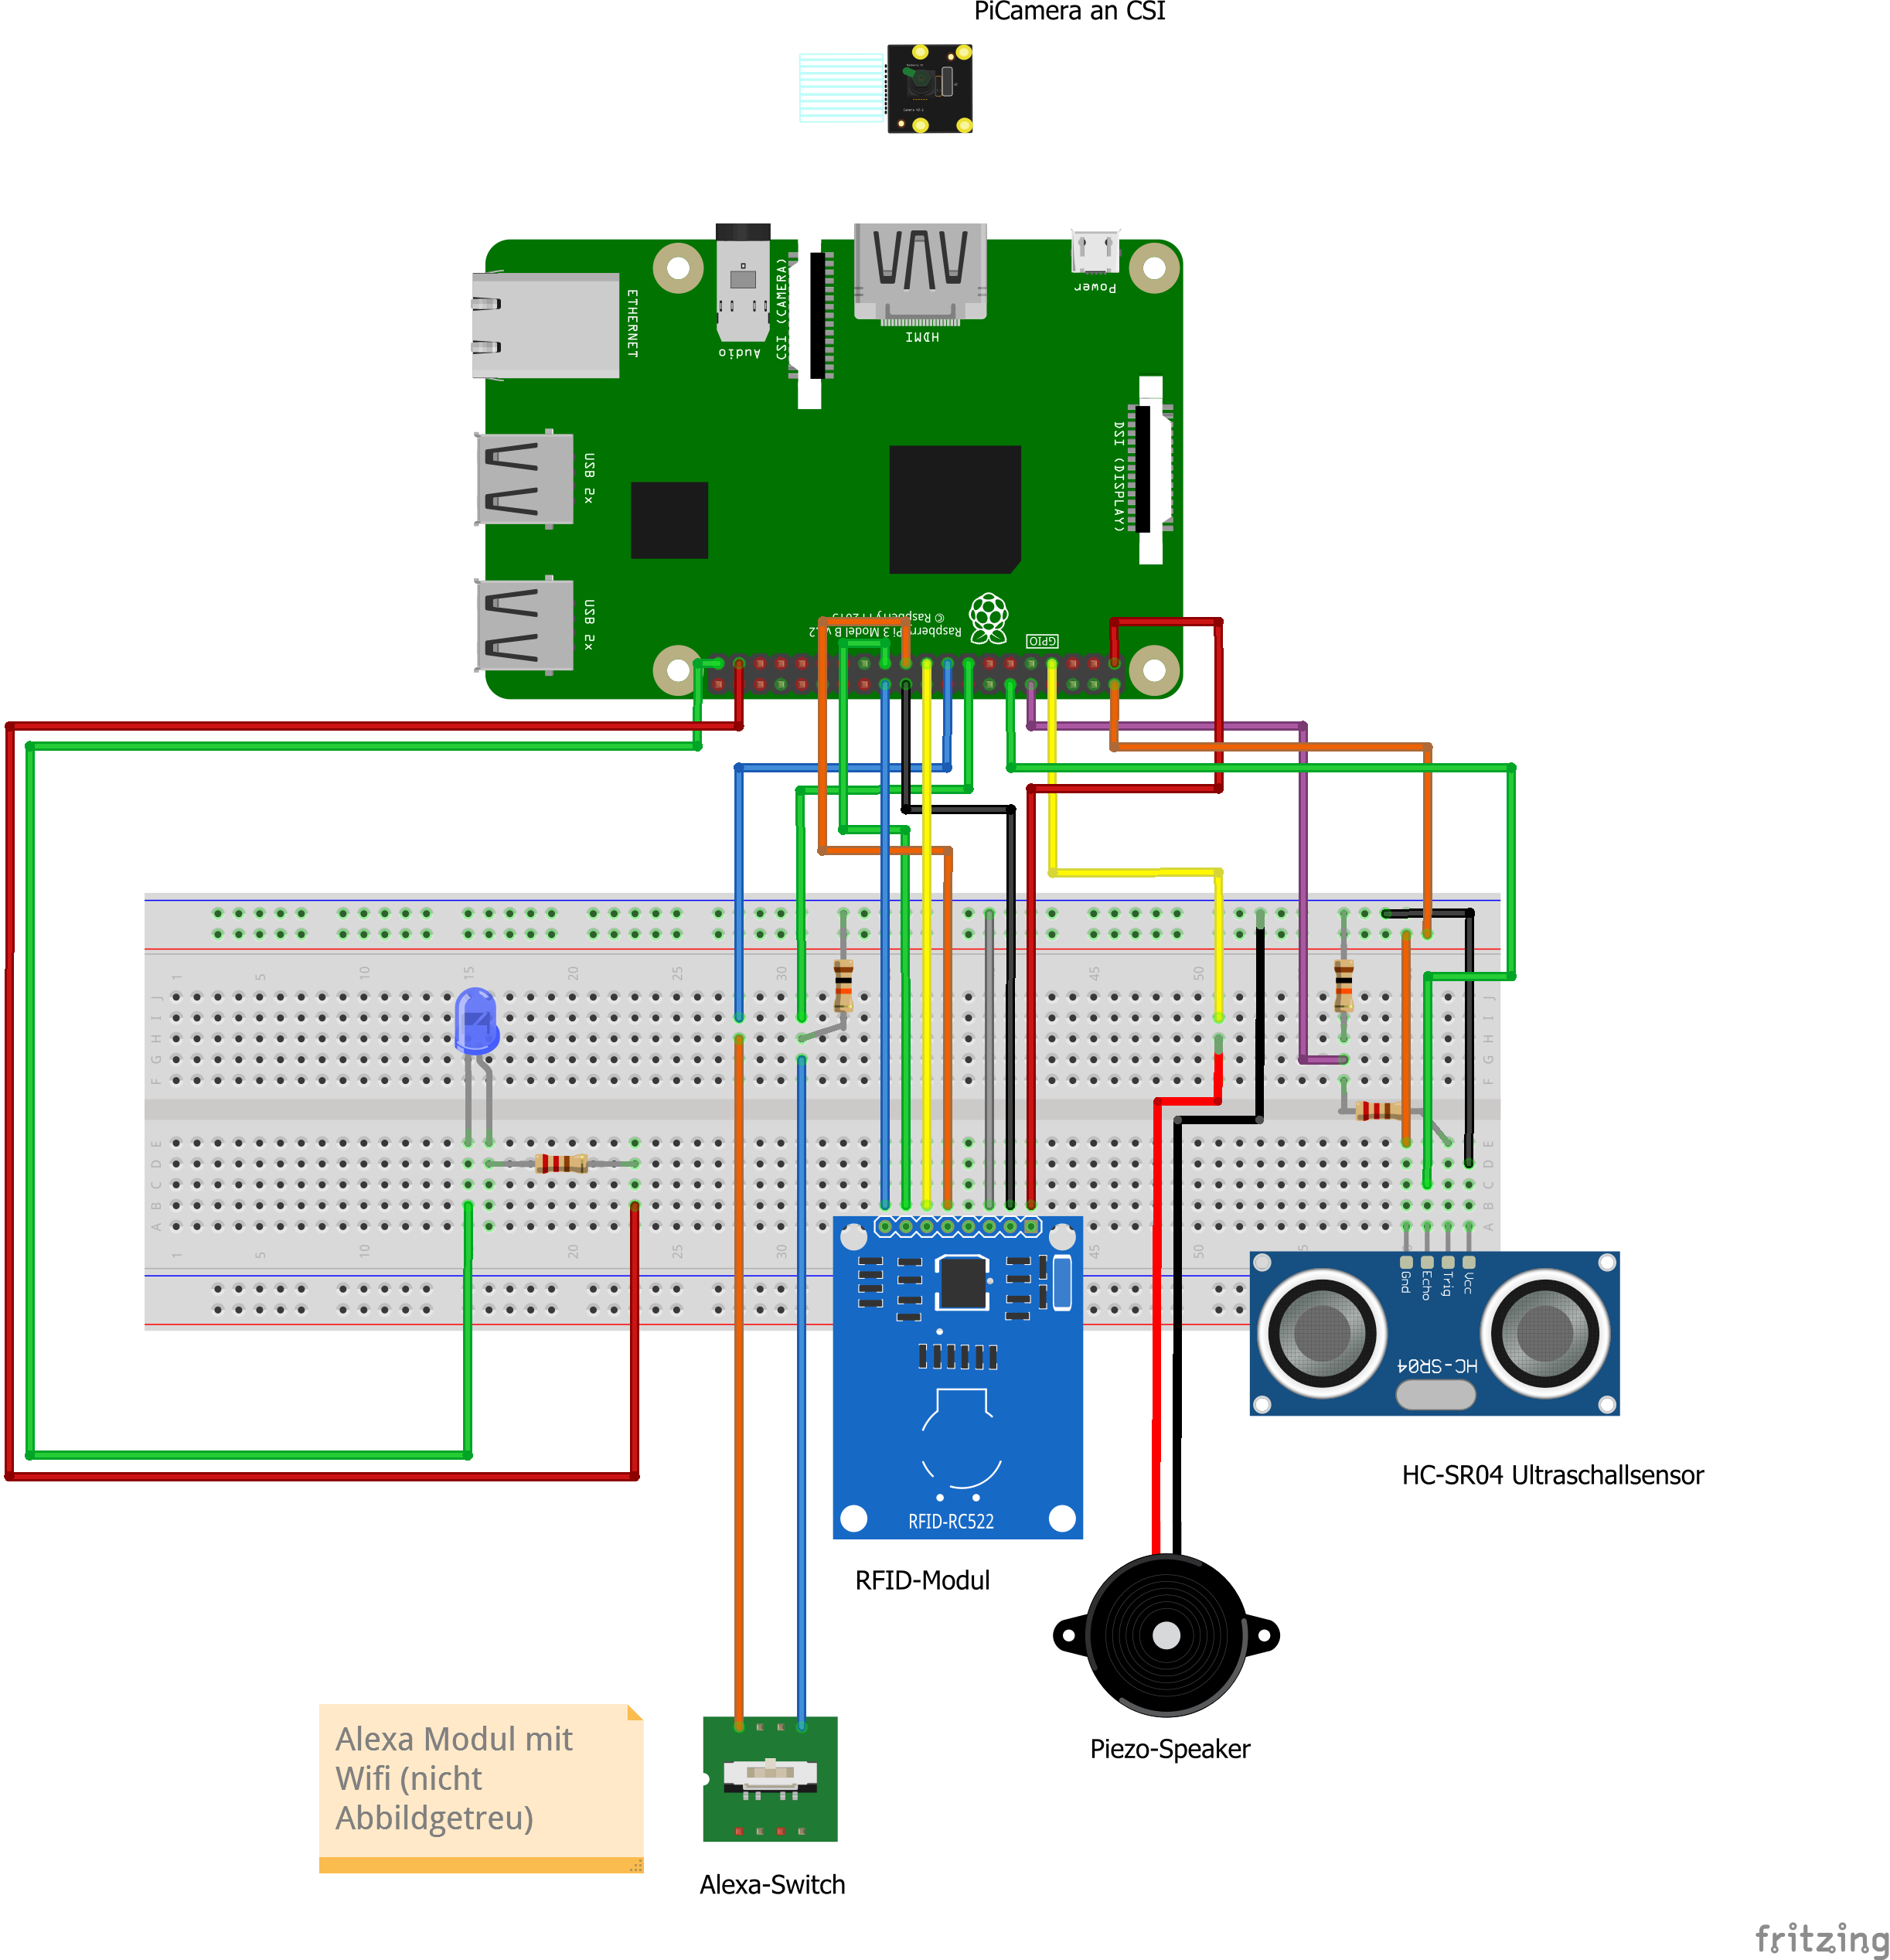
\includegraphics[scale=0.5]{\imagedir/SmartGarage.png}
	\captionsetup{format=hang}
	\caption[Steckplan]{\label{Steckplansm}Steckplan der gesamten Hardware \\Quelle: Eigene Darstellung}
\end{figure}
\begin{figure}
	\centering 
	\label{}
	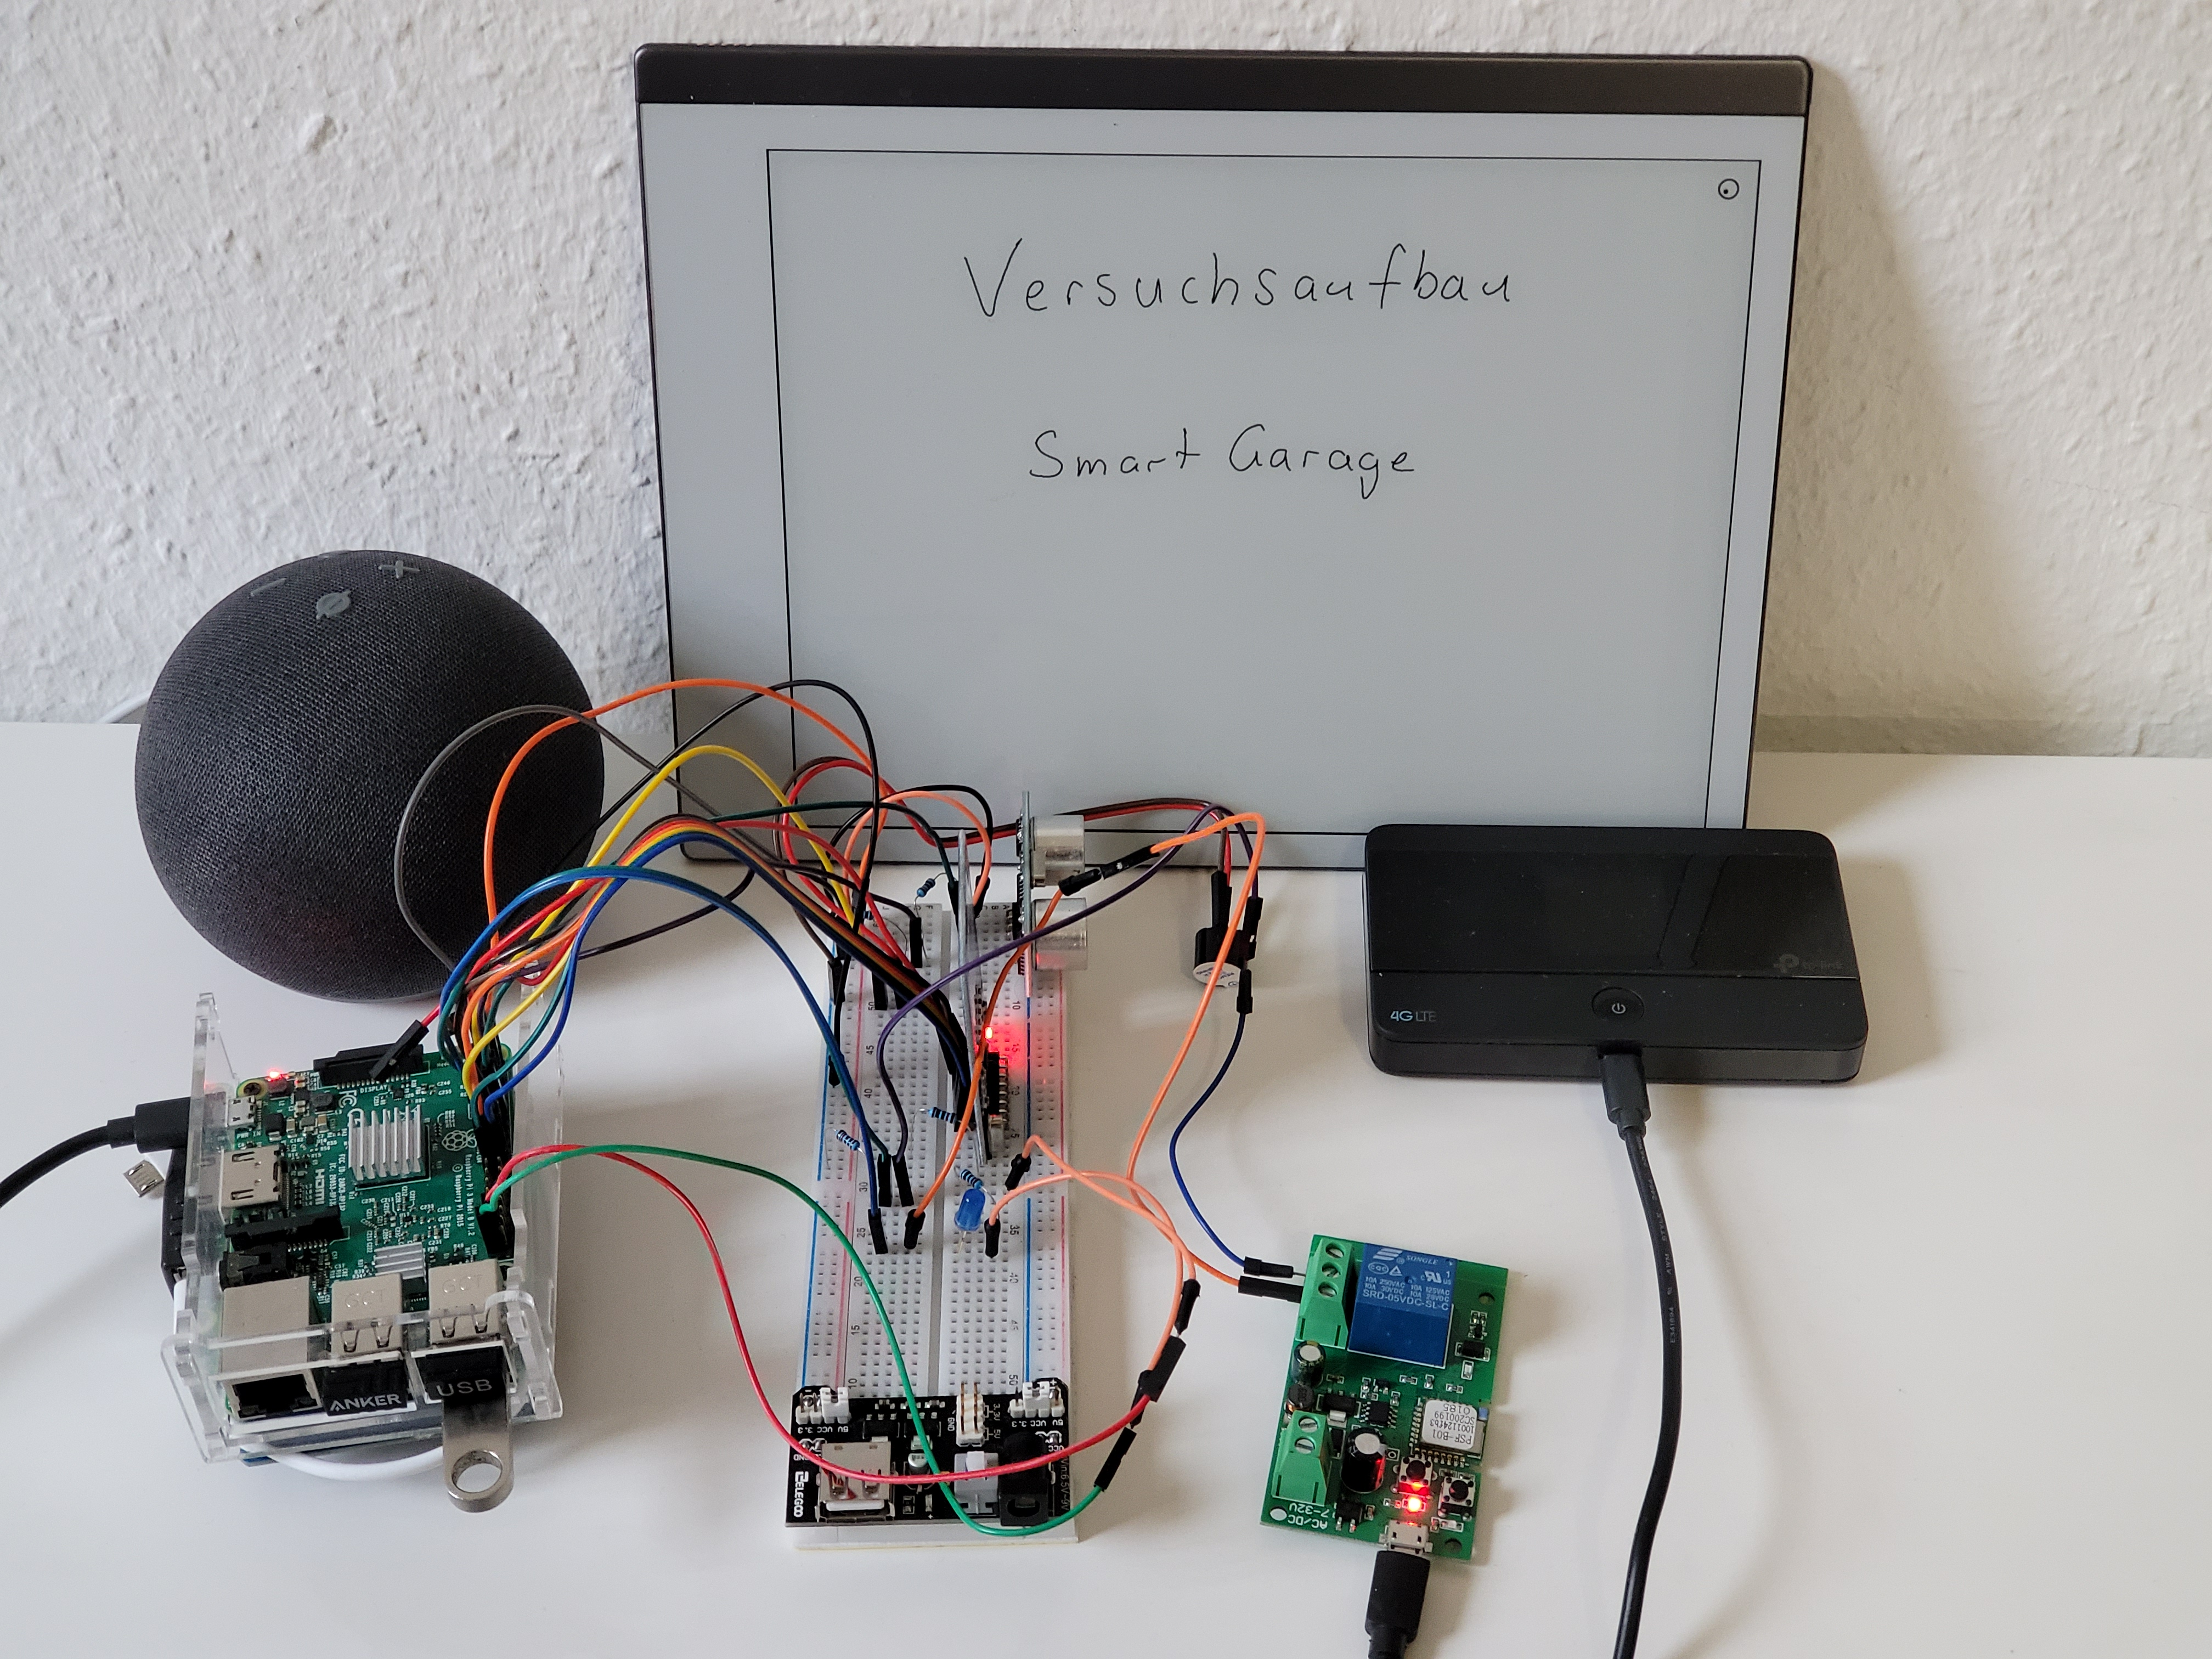
\includegraphics[scale=0.08]{\imagedir/Foto (7).jpg}
	\captionsetup{format=hang}
	\caption[Versuchsaufbau]{\label{Aufbau1}Fertiger Aufbau aller Module\\Quelle: Eigene Darstellung}
\end{figure}
\chapter{Risiken und Limitierungen}

Mehrere problematische Punkte konnten innerhalb der relativ kurzen Projektlaufzeit noch nicht ausreichend adressiert werden. Sie wurden aber erfasst und in diesem kurzen Abschnitt notiert.

Zum einen hat die verwendete Software noch Schwierigkeiten mit Störungen durch Fahrzeug- und Kennzeichenhalterbeschriftungen und deutsche Umlaute, die in manchen Kennzeichen vorhanden sind, können noch nicht erkannt werden. Dies war auf den erfassten Testdaten in Mannheim/Heidelberg nicht nicht problematisch, wird es aber für andere Regionen sein.
Zum anderen ergeben sich durch die optische Erkennung naturgemäß etliche Probleme bei erschwerten Sichtverhältnissen wie Schnee, Regen, Dunkelheit oder schlicht verschmutzten Kennzeichen. 

Ein weiterer bedeutender Punkt ist die mangelnde Sicherheit des Systems. Da die Öffnung des Garagentors nur durch das Kennzeichen geschieht, ist das Missbrauchs-bzw. Einbruchspotenzial groß. Im schlimmsten Fall reicht ein bedrucktes DIN-A4 Blatt mit dem richtigen Kennzeichen um die Garage zu öffnen. Auch Hackerangriffe sind prinzipiell möglich.

Ebenfalls sollte bei der Installation der Datenschutz beachtet werden. So ist es nicht erlaubt öffenliche Bereiche zu filmen.

Eine Messung des Stromverbrauchs hat nicht stattgefunden, dementsprechend kann auch keine Aussage über die laufenden Betriebskosten des RasPi mit allen Modulen und der Luxonis-Kamera getätigt werden.

\chapter{Wirtschaftliche Aspekte}
Auch wenn die technische Konzeption und Umsetzung im Mittelpunkt dieser Arbeit stehen, soll aufgrund der Ausrichtung des Studiengangs hier auch kurz auf einige betriebswirtschaftliche Aspekte des Projekts eingegangen werden.\subparagraph*{Entwicklungskosten}
   \newline
Zeitaufwand pro Teammitglied

\begin{tabular}[h]{lcr}
2x Projektkonzeption/Kick-Off online 2 Stunden \\
3x Workshops a 12 Stunden\\
2x Workshop a 8 Stunden\\
1x Praxistest 4 Stunden\\
1x Abschluss-Workshop a 24 Stunden \\
8 Stunden Ausarbeitung Projektbericht / Dokumentation\\
\end{tabular} \newline

Bei einem angenommenen Stundenlohn von 15€, der für Werkstudenten mit vergleichbaren Kenntnissen angemessen ist, ergeben sich bei den aufsummierten 368 Mannstunden geschätzte kalkulatorische Entwicklungskosten von 5520€
\subparagraph*{Materialkosten} in Euro, inkl. Versand  \newline 

\begin{tabular}[h]{lcr}
Raspberry Pi 3	&   39,95 \autocite{Pi3b} \newline \\
RFID-Modul RC552 &		5,00\autocite{RFID} \newline\\
Ultraschallmodul	&  8,94\autocite{SR04} \newline \\
Amazon Alexa Wifi Modul & 13,99\autocite{eWe}	\\
OAK-D Kamera & 185,51 \autocite{eWe} \\
\textbf{Summe}			&	\textbf{253,39}
\end{tabular} \newline


Die geschätzte Installationszeit pro Einheit für Verkabelung des Kameramoduls und des RasPi, Befestigung des RFID-Sensors, Ausrichtung der Kamera und Tests beträgt für einen geübten Elektriker ca. 4 Stunden.
Bei einem angenommenen Kosten von 60€/Stunde wären dies 240€ (ohne Anfahrt). Der Verkaufspreis inklusive Installation müsste also mindestens bei knapp 500€ liegen, um einen Deckungskostenbeitrag zu erzielen und die Entwicklungskosten von 5520€ zu decken.




